% ============================================================
%  Chapter 21 --- Uncertainty Propagation
%  Algorithms for Optimization, 2nd ed. (2026)
%  Kochenderfer & Wheeler
% ============================================================
\documentclass[aspectratio=169,10pt]{beamer}

\usetheme{Madrid}
\usecolortheme{seahorse}

\usepackage[utf8]{inputenc}
\usepackage[T1]{fontenc}
\usepackage{amsmath,amssymb,mathtools}
\usepackage{bm}
\usepackage{booktabs}
\usepackage{graphicx}
\usepackage{listings}
\usepackage{xcolor}
\usepackage{array}
\usepackage{tikz}
\usetikzlibrary{positioning,shapes.geometric}
\usepackage{pgfplots}
\pgfplotsset{compat=1.18}

\graphicspath{{figures/}}

\setbeamertemplate{footline}[frame number]
\setbeamertemplate{navigation symbols}{}

% -- Python listings style ----------------------------------
\lstset{
  language=Python,
  basicstyle=\ttfamily\scriptsize,
  numbers=left,
  numberstyle=\tiny\color{gray},
  frame=single,
  backgroundcolor=\color{gray!7},
  keywordstyle=\color{blue!70!black}\bfseries,
  commentstyle=\color{green!50!black}\itshape,
  stringstyle=\color{orange!80!black},
  breaklines=true,
  showstringspaces=false,
  tabsize=4,
  xleftmargin=2em,
  numbersep=5pt,
}

% -- Convenience macros ------------------------------------
\newcommand{\bx}{\mathbf{x}}
\newcommand{\bz}{\mathbf{z}}
\newcommand{\bmu}{\boldsymbol{\mu}}
\newcommand{\bSigma}{\boldsymbol{\Sigma}}
\newcommand{\E}{\mathbb{E}}
\newcommand{\Var}{\mathrm{Var}}
\newcommand{\R}{\mathbb{R}}
\newcommand{\hmu}{\hat{\mu}}
\newcommand{\hnu}{\hat{\nu}}
\newcommand{\hf}{\hat{f}}

% -- Title -------------------------------------------------
\title[Ch.\ 21: Uncertainty Propagation]{Chapter 21\\[4pt]
  \textbf{Uncertainty Propagation}}
\subtitle{Algorithms for Optimization, 2nd ed.\ (2026)\\
  Kochenderfer \& Wheeler}
\author{Lecture Slides}
\date{}

% ============================================================
\begin{document}
% ============================================================

\begin{frame}
  \titlepage
\end{frame}

% -- Table of Contents -------------------------------------
\begin{frame}{Chapter Overview}
  \tableofcontents
\end{frame}

% ============================================================
\section{Introduction}
% ============================================================

\begin{frame}{Motivation: Uncertainty in Optimization}
  \begin{columns}[T]
    \column{0.55\textwidth}
      \begin{block}{Problem Setting}
        In probabilistic optimization under uncertainty,
        some inputs to the objective $f(\bx,\bz)$ are
        modelled as a \textbf{random variable} $\bz\sim p(\bz)$
        over domain $\mathcal{Z}$.
      \end{block}
      \vspace{0.5em}
      \textbf{Goal:} propagate the known input distribution $p(\bz)$
      to estimate quantities of the \emph{output} distribution:
      \begin{itemize}
        \item Expected value $\;\E_{\bz\sim p}[f(\bz)]$
        \item Variance $\;\Var_{\bz\sim p}[f(\bz)]$
      \end{itemize}
      \vspace{0.5em}
      \textbf{Note:} for brevity we drop $\bx$ from $f(\bx,\bz)$;
      the dependency still exists and we recompute per design point.

    \column{0.42\textwidth}
      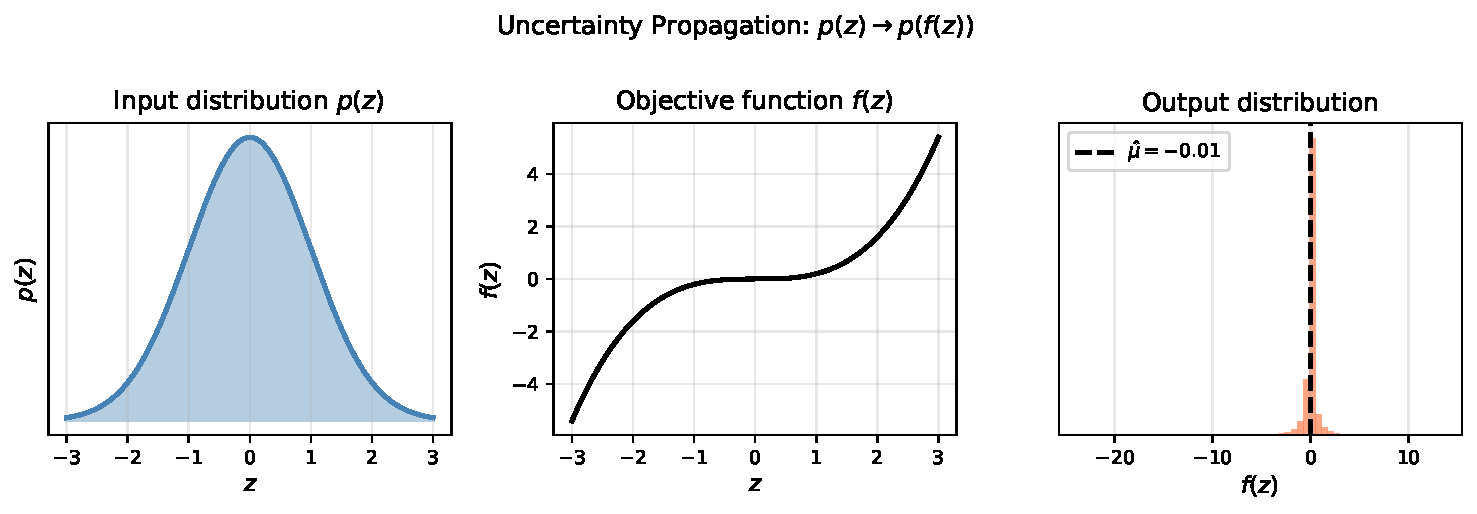
\includegraphics[width=\linewidth]{overview}
  \end{columns}
\end{frame}

\begin{frame}{Methods Covered}
  \begin{columns}[T]
    \column{0.50\textwidth}
      \begin{block}{Four Approaches}
        \begin{enumerate}
          \item \textbf{Monte Carlo Sampling}\\
                No derivatives; black-box; slow convergence
          \item \textbf{Taylor Approximation}\\
                Requires derivatives; analytic; fast
          \item \textbf{Polynomial Chaos}\\
                Surrogate model; orthogonal basis fit
          \item \textbf{Bayesian Monte Carlo}\\
                GP surrogate; analytic for Gaussian inputs
        \end{enumerate}
      \end{block}
    \column{0.46\textwidth}
      \begin{block}{Key quantities}
        $f(\bz)$: objective function\\
        $p(\bz)$: known input distribution\\
        $\hmu$: estimated mean\\
        $\hnu$: estimated variance
      \end{block}
      \begin{alertblock}{Trade-offs}
        Accuracy \textit{vs.}\ computational cost\\
        \#~function evaluations needed\\
        Assumptions on $f$ smoothness
      \end{alertblock}
  \end{columns}
\end{frame}

% ============================================================
\section{21.1 Sampling Methods (Monte Carlo)}
% ============================================================

\begin{frame}{21.1 Monte Carlo Sampling}
  \begin{block}{Sample Mean and Sample Variance (Eqs.\ 21.1--21.2)}
    Draw $m$ i.i.d.\ samples $\bz^{(1)},\ldots,\bz^{(m)} \sim p(\bz)$:
    \[
      \E_{\bz\sim p}[f(\bz)] \;\approx\; \hmu
        = \frac{1}{m}\sum_{i=1}^{m} f\!\left(\bz^{(i)}\right)
    \]
    \[
      \Var_{\bz\sim p}[f(\bz)] \;\approx\; \hnu
        = \left(\frac{1}{m}\sum_{i=1}^{m} f\!\left(\bz^{(i)}\right)^{\!2}\right) - \hmu^2
    \]
    \smallskip
    \begin{tabular}{ll}
      $m$ & number of samples\\
      $\bz^{(i)}$ & $i$-th sample from $p$\\
      $\hmu$ & sample mean (estimator of $\E[f]$)\\
      $\hnu$ & sample variance (estimator of $\Var[f]$)
    \end{tabular}
  \end{block}
\end{frame}

\begin{frame}{Monte Carlo: Convergence Properties}
  \begin{columns}[T]
    \column{0.52\textwidth}
      \begin{block}{Variance of the estimator}
        For normally distributed $f$:
        \[
          \Var[\hmu] = \frac{\nu}{m}
        \]
        Doubling $m$ \emph{halves} the variance.\\
        \medskip
        Convergence rate: $\mathcal{O}(m^{-1/2})$
      \end{block}
      \medskip
      \textbf{Advantages:}
      \begin{itemize}
        \item $p$ need not be known exactly
        \item Works with simulation / real experiments
        \item No smoothness assumptions on $f$
      \end{itemize}
      \textbf{Limitation:}
      \begin{itemize}
        \item Slow convergence; many evaluations needed
        \item Quasi-MC (Ch.~16) gives faster convergence
      \end{itemize}
    \column{0.45\textwidth}
      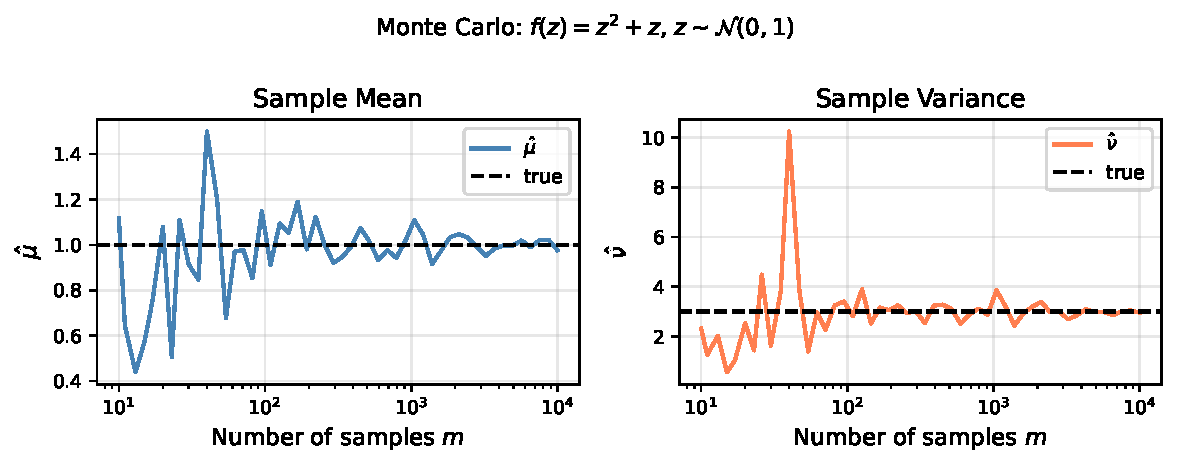
\includegraphics[width=\linewidth]{mc_convergence}
      \vspace{-1em}
      \begin{center}\small $f(z)=z^2+z$, $z\sim\mathcal{N}(0,1)$\end{center}
  \end{columns}
\end{frame}

\begin{frame}[fragile]{Monte Carlo in Python}
\begin{lstlisting}
import numpy as np

def monte_carlo_moments(f, sample_fn, m=10000, seed=42):
    """
    Estimate mean and variance of f(z) using Monte Carlo.
    Parameters
    ----------
    f         : callable, objective function f(z)
    sample_fn : callable, draws 1 sample from p(z)
    m         : int, number of samples
    Returns
    -------
    mu_hat, nu_hat : float, estimated mean and variance
    """
    rng = np.random.default_rng(seed)
    samples = np.array([f(sample_fn(rng)) for _ in range(m)])
    mu_hat = np.mean(samples)
    nu_hat = np.mean(samples**2) - mu_hat**2
    return mu_hat, nu_hat

# Example: f(z) = sin(z), z ~ N(0,1)
f = np.sin
sample_fn = lambda rng: rng.standard_normal()

mu, nu = monte_carlo_moments(f, sample_fn, m=5000)
print(f"mu_hat = {mu:.4f}")   # -> ~0.0
print(f"nu_hat = {nu:.4f}")   # -> ~0.4597
\end{lstlisting}
\end{frame}

% ============================================================
\section{21.2 Taylor Approximation}
% ============================================================

\begin{frame}{21.2 Taylor Approximation --- Setup}
  \begin{block}{Second-Order Taylor Expansion of $f(\bz)$ at $\bz=\bmu_z$}
    \[
      \hf(\bz) = f(\bmu_z)
        + \sum_{i=1}^{n}\frac{\partial f}{\partial z_i}(z_i-\mu_i)
        + \frac{1}{2}\sum_{i=1}^{n}\sum_{j=1}^{n}
          \frac{\partial^2 f}{\partial z_i\partial z_j}(z_i-\mu_i)(z_j-\mu_j)
    \]
  \end{block}

  \textbf{Assumptions:}
  \begin{itemize}
    \item Components of $\bz$ are \textbf{uncorrelated} (or whitened)
    \item Each $z_i$ has mean $\mu_i$ and variance $\nu_i$
    \item All derivatives evaluated at $\bz = \bmu_z$
  \end{itemize}

  \begin{block}{Whitening correlated inputs}
    If $\bz=\mathbf{c}$ with covariance $\mathbf{C}$, transform:
    $\bz = \mathbf{T}\mathbf{c}$,
    where $\mathbf{T}$ contains the eigenvectors of $\mathbf{C}$
    (columns ordered by the $m$ largest eigenvalues).
  \end{block}
\end{frame}

\begin{frame}{Taylor Approximation --- Mean and Variance Formulas}
  \begin{block}{Second-Order Estimates (Eqs.\ 21.4--21.5)}
    \[
      \hmu = f(\bmu_z)
        + \frac{1}{2}\sum_{i=1}^{n}
          \frac{\partial^2 f}{\partial z_i^2}\,\nu_i
        \;\Bigg|_{\bz=\bmu_z}
    \]
    \[
      \hnu = \sum_{i=1}^{n}\left(\frac{\partial f}{\partial z_i}\right)^{\!2}\!\nu_i
           + \frac{1}{2}\sum_{i=1}^{n}\sum_{j=1}^{n}
             \left(\frac{\partial^2 f}{\partial z_i\partial z_j}\right)^{\!2}\!\nu_i\nu_j
        \;\Bigg|_{\bz=\bmu_z}
    \]
  \end{block}

  \begin{block}{First-Order Approximation (Eq.\ 21.6) --- Simpler}
    \[
      \hmu \approx f(\bmu_z),\qquad
      \hnu \approx \sum_{i=1}^{n}\left(\frac{\partial f}{\partial z_i}\right)^{\!2}\!\nu_i
        \;\Bigg|_{\bz=\bmu_z}
    \]
    Neglects higher-order terms; efficient when $f$ is nearly linear.
  \end{block}
  \textbf{Symbol guide:}
  $\nu_i = \Var[z_i]$, $\;\bmu_z = \E[\bz]$,
  $\;n$ = dimension of $\bz$.
\end{frame}

\begin{frame}{Taylor Approximation --- Numerical Example}
  \begin{block}{Example 21.1: $f(x,z)=\sin(x+z_1)\cos(x+z_2)$}
    $z_1\sim\mathcal{N}(0,0.1)$, $z_2\sim\mathcal{N}(0,0.2)$;
    evaluate at $\bmu_z=(0,0)$.
    \medskip

    \textbf{Partial derivatives at $\bz=\mathbf{0}$:}
    \quad$\dfrac{\partial f}{\partial z_1}=\cos(x)\cos(x)$,\quad
    $\dfrac{\partial f}{\partial z_2}=-\sin(x)\sin(x)$

    \medskip
    \textbf{Resulting approximations:}
    \[
      \hmu(x) = 0.85\sin(x)\cos(x),\quad
      \hnu(x) = 0.1\cos^4(x)+0.2\sin^4(x)+0.045\sin^2(x)\cos^2(x)
    \]
  \end{block}
\end{frame}

\begin{frame}{Taylor Approximation --- Results}
  \begin{columns}[T]
    \column{0.55\textwidth}
      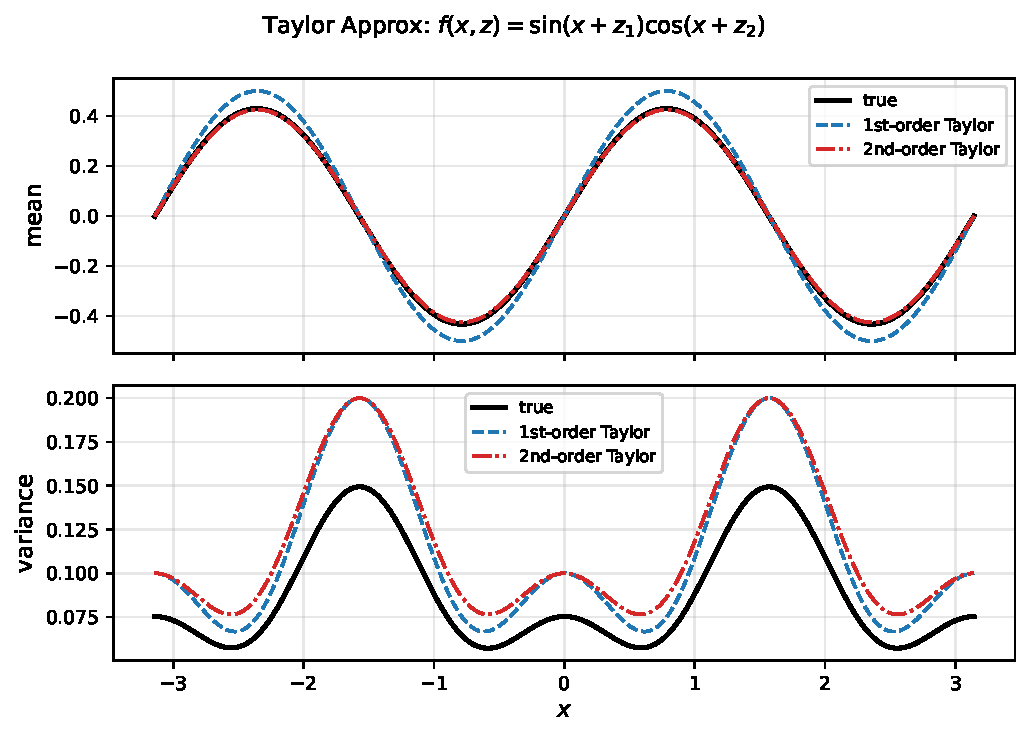
\includegraphics[width=\linewidth]{taylor_approx}
    \column{0.42\textwidth}
      \begin{block}{Observations}
        \begin{itemize}
          \item \textbf{1st-order} mean: $\hmu\approx f(\bmu_z)$
                (ignores curvature correction)
          \item \textbf{2nd-order} mean adds a bias correction
                proportional to the Hessian diagonal
          \item Variance quality depends on the nonlinearity of $f$
        \end{itemize}
      \end{block}
      \begin{alertblock}{When to use}
        Best when $f$ is smooth and the noise variances
        $\nu_i$ are small relative to the function's length scale.
      \end{alertblock}
  \end{columns}
\end{frame}

\begin{frame}[fragile]{Taylor Approximation in Python}
\begin{lstlisting}
import numpy as np

def taylor_approx(f, mu_z, nu_z, second_order=False, eps=1e-5):
    """Estimate mean and variance via Taylor approximation."""
    mu_z = np.asarray(mu_z, float); nu_z = np.asarray(nu_z, float)
    n = len(mu_z); f0 = f(mu_z)
    # Numerical gradient
    grad = np.array([(f(mu_z+np.eye(n)[i]*eps)-f(mu_z-np.eye(n)[i]*eps))/(2*eps)
                      for i in range(n)])
    mu_hat = f0
    nu_hat = np.dot(grad**2, nu_z)
    if second_order:
        hess_d = np.array([(f(mu_z+np.eye(n)[i]*eps)-2*f0+f(mu_z-np.eye(n)[i]*eps))/eps**2
                            for i in range(n)])
        mu_hat += 0.5 * np.dot(hess_d, nu_z)
        nu_hat += 0.5 * np.dot(hess_d**2, nu_z**2)
    return mu_hat, nu_hat

# Example 21.1: f(x,z) = sin(x+z[0])*cos(x+z[1])
x = 0.5
f = lambda z: np.sin(x+z[0]) * np.cos(x+z[1])
mu_z, nu_z = [0.0, 0.0], [0.1, 0.2]
mu1, nu1 = taylor_approx(f, mu_z, nu_z, second_order=False)
mu2, nu2 = taylor_approx(f, mu_z, nu_z, second_order=True)
print(f"1st: mu={mu1:.4f}, nu={nu1:.4f}")
print(f"2nd: mu={mu2:.4f}, nu={nu2:.4f}")
\end{lstlisting}
\end{frame}

% ============================================================
\section{21.3 Polynomial Chaos}
% ============================================================

\begin{frame}{21.3 Polynomial Chaos --- Idea}
  \begin{columns}[T]
    \column{0.58\textwidth}
      \begin{block}{Surrogate Model (Eq.\ 21.7)}
        Approximate $f(z)$ with $k$ polynomial basis functions:
        \[
          f(z) \;\approx\; \hf(z) = \sum_{i=1}^{k}\theta_i b_i(z)
        \]
        $\theta_i$: coefficients to fit\\
        $b_i(z)$: basis polynomials (degree $i-1$, $b_1=1$)
      \end{block}
      \medskip
      \textbf{Workflow:}
      \begin{enumerate}
        \item Choose basis polynomials orthogonal under $p(z)$
        \item Fit coefficients $\theta_i$ to function evaluations
        \item Read off mean and variance analytically
      \end{enumerate}
    \column{0.38\textwidth}
      \begin{alertblock}{Key insight}
        With \emph{orthogonal} bases:
        \[
          \hmu = \theta_1
        \]
        \[
          \hnu = \sum_{i=2}^{k}\theta_i^2
                 \int_{\mathcal{Z}} b_i(z)^2 p(z)\,dz
        \]
        No numerical integration needed for $\hmu$!
      \end{alertblock}
  \end{columns}
\end{frame}

\begin{frame}{Orthogonality and Mean/Variance Derivation}
  \begin{block}{Orthogonality Condition (Eq.\ 21.20)}
    Two basis functions $b_i$ and $b_j$ are \textbf{orthogonal} w.r.t.\ $p(z)$ if:
    \[
      \int_{\mathcal{Z}} b_i(z)\,b_j(z)\,p(z)\,dz = 0 \quad (i\ne j)
    \]
  \end{block}
  \begin{columns}[T]
    \column{0.48\textwidth}
      \begin{block}{Mean (Eqs.\ 21.21--21.24)}
        With $b_1(z)=1$ and all bases orthogonal:
        \[
          \hmu = \theta_1 \int_{\mathcal{Z}} p(z)\,dz = \theta_1
        \]
        (since all cross-terms vanish)
      \end{block}
    \column{0.48\textwidth}
      \begin{block}{Variance (Eqs.\ 21.25--21.28)}
        \[
          \hnu = \sum_{i=2}^{k}\theta_i^2 \int_{\mathcal{Z}} b_i(z)^2 p(z)\,dz
        \]
        Cross-terms vanish by orthogonality.\\
        These integrals can be precomputed!
      \end{block}
  \end{columns}
\end{frame}

\begin{frame}{Orthogonal Basis Functions --- Standard Families}
  \begin{center}
    \small
    \begin{tabular}{llllp{3cm}}
      \toprule
      Distribution & Domain & Density & Basis & Recurrence\\
      \midrule
      Uniform & $[-1,1]$ & $\tfrac{1}{2}$ & Legendre &
        $\tfrac{2i-3}{i-1}z\,b_{i-1} - \tfrac{i-2}{i-1}b_{i-2}$\\[4pt]
      Exponential & $[0,\infty)$ & $e^{-z}$ & Laguerre &
        $\tfrac{1}{i-1}\bigl((2i-3-z)b_{i-1}-(i-2)b_{i-2}\bigr)$\\[4pt]
      Unit Gaussian & $(-\infty,\infty)$ & $\tfrac{1}{\sqrt{2\pi}}e^{-z^2/2}$ & Hermite &
        $z\,b_{i-1}(z) - \tfrac{d}{dz}b_{i-1}(z)$\\
      \bottomrule
    \end{tabular}
    \vspace{0.3em}

    \textit{Table 21.1: Orthogonal polynomial basis functions}
  \end{center}

  \vspace{0.3em}
  \begin{columns}[T]
    \column{0.55\textwidth}
      \textbf{Three-term recurrence (Eq.\ 21.29):}
      \[
        b_{i+1}(z) = \begin{cases}
          (z-\alpha_i)b_i(z) & i=1\\
          (z-\alpha_i)b_i(z)-\beta_i b_{i-1}(z) & i>1
        \end{cases}
      \]
    \column{0.42\textwidth}
      with $b_1(z)=1$ and weights:
      \[
        \alpha_i = \frac{\int z\,b_i^2 p\,dz}{\int b_i^2 p\,dz},\quad
        \beta_i  = \frac{\int b_i^2 p\,dz}{\int b_{i-1}^2 p\,dz}
      \]
  \end{columns}
\end{frame}

\begin{frame}{Orthogonal Basis Functions --- Plots}
  \begin{center}
    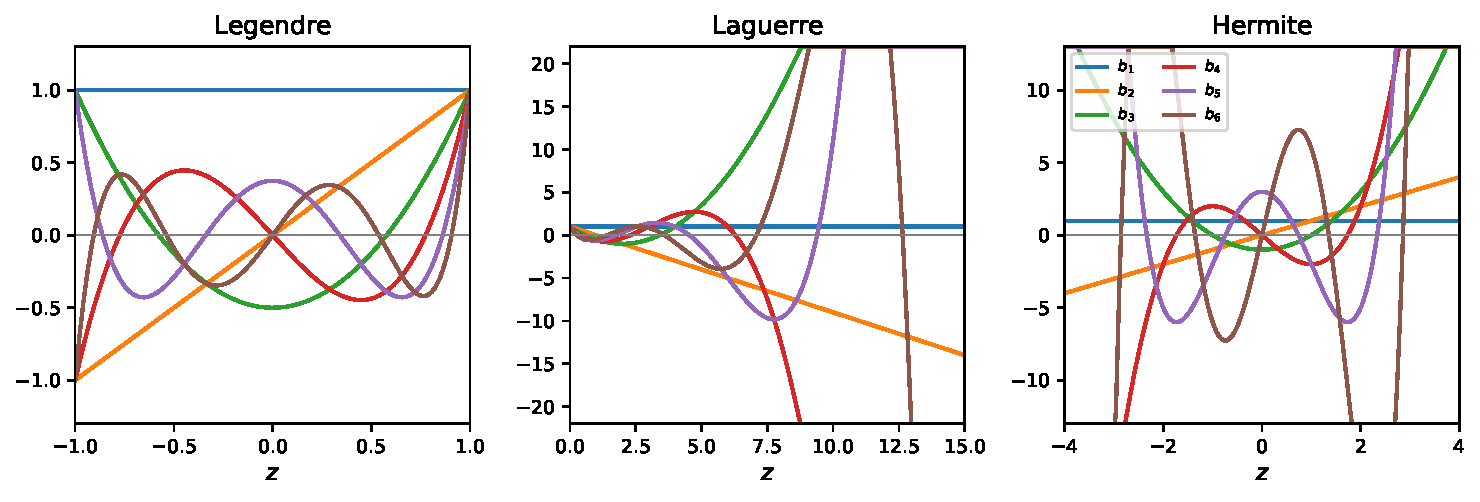
\includegraphics[width=0.95\linewidth]{orthogonal_bases}
  \end{center}
  \vspace{-0.5em}
  \begin{center}\small Figure 21.1: Legendre (uniform), Laguerre (exponential),
  Hermite (unit Gaussian) basis functions $b_1,\ldots,b_6$.\end{center}
\end{frame}

\begin{frame}{21.3.2 Fitting the Coefficients}
  \begin{block}{Method 1: Linear Regression}
    Given samples $z^{(1)},\ldots,z^{(m)}$ and values $f(z^{(i)})$,
    solve the least-squares problem:
    \[
      \underbrace{\begin{bmatrix}b_1(z^{(1)}) & \cdots & b_k(z^{(1)})\\
        \vdots & \ddots & \vdots\\
        b_1(z^{(m)}) & \cdots & b_k(z^{(m)})\end{bmatrix}}_{\mathbf{B}}
      \underbrace{\begin{bmatrix}\theta_1\\\vdots\\\theta_k\end{bmatrix}}_{\bm{\theta}}
      \approx
      \underbrace{\begin{bmatrix}f(z^{(1)})\\\vdots\\f(z^{(m)})\end{bmatrix}}_{\mathbf{y}}
    \]
  \end{block}

  \begin{block}{Method 2: Gauss Quadrature (Eq.\ 21.38)}
    Exploit orthogonality to obtain the $j$-th coefficient directly:
    \[
      \theta_j = \frac{\displaystyle\int_{\mathcal{Z}} f(z)\,b_j(z)\,p(z)\,dz}
                      {\displaystyle\int_{\mathcal{Z}} b_j(z)^2\,p(z)\,dz}
    \]
    The denominator is precomputed; the numerator is evaluated by Gaussian quadrature.
  \end{block}
\end{frame}

\begin{frame}[fragile]{Polynomial Chaos in Python --- Legendre Fit}
\begin{lstlisting}
import numpy as np
from scipy.special import legendre as sp_legendre
from scipy import integrate

def poly_chaos_legendre(z_samples, f_samples, k):
    """
    Fit k Legendre basis functions and return (theta, mu_hat, nu_hat).
    Assumes z ~ Uniform[-1,1], p(z) = 1/2.
    """
    # Build Vandermonde matrix B[i,j] = P_j(z_i)
    B = np.column_stack([sp_legendre(j)(z_samples) for j in range(k)])
    # Least-squares fit
    theta, _, _, _ = np.linalg.lstsq(B, f_samples, rcond=None)
    mu_hat = theta[0]   # = theta_1 since b_1 = P_0 = 1
    # Var: sum_{j>=1} theta_j^2 * integral P_j^2(z)*(1/2)dz
    # integral_{-1}^{1} P_j^2(z)/2 dz = 1/(2j+1)
    nu_hat = sum(theta[j]**2 / (2*j+1) for j in range(1, k))
    return theta, mu_hat, nu_hat

# Example 21.3: f(z) = sin(pi*z), 5 samples
z_s = np.array([-1.0, -0.2, 0.3, 0.7, 0.9])
y_s = np.sin(np.pi * z_s)

for k in range(1, 6):
    _, mu, nu = poly_chaos_legendre(z_s, y_s, k)
    print(f"k={k}: mu_hat={mu:+.3f}, nu_hat={nu:.3f}")
# True: mu=0, nu=0.5
\end{lstlisting}
\end{frame}

\begin{frame}{Example 21.3 --- Legendre Fit to $\sin(\pi z)$}
  \begin{columns}[T]
    \column{0.55\textwidth}
      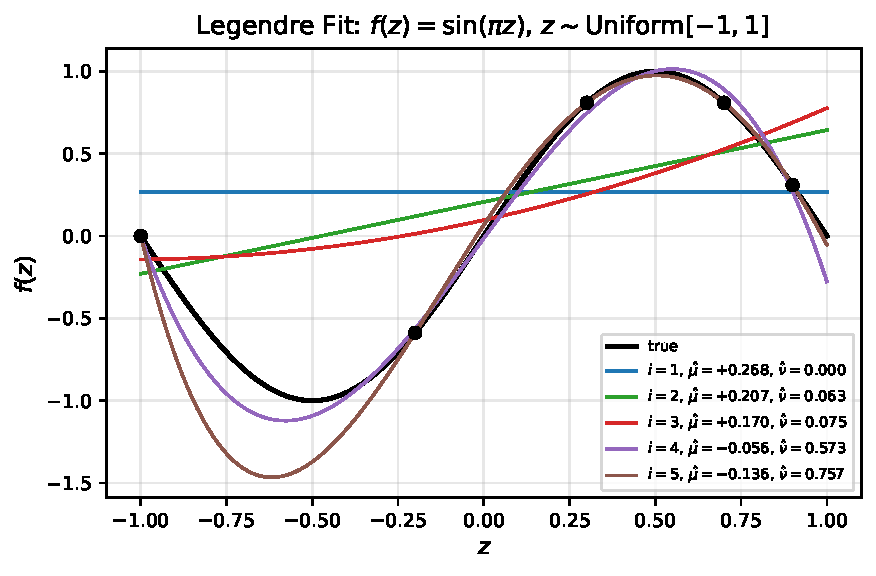
\includegraphics[width=\linewidth]{legendre_fit}
    \column{0.42\textwidth}
      \begin{block}{Setup}
        $f(z)=\sin(\pi z)$, $z\sim\mathrm{Unif}[-1,1]$\\
        True: $\mu=0$, $\nu=0.5$\\
        Five samples: $\{-1,{-}0.2,0.3,0.7,0.9\}$
      \end{block}
      \begin{block}{Results by degree}
        \small
        \begin{tabular}{lrr}
          \toprule
          $i$ & $\hmu$ & $\hnu$\\
          \midrule
          1 & $+0.268$ & 0.000\\
          2 & $+0.207$ & 0.063\\
          3 & $+0.170$ & 0.075\\
          4 & $-0.056$ & 0.573\\
          5 & $-0.136$ & 0.757\\
          \bottomrule
        \end{tabular}
      \end{block}
      Higher degree $\to$ overfitting with only 5 points.
  \end{columns}
\end{frame}

\begin{frame}{21.3.1 Stieltjes Algorithm --- Arbitrary Distributions}
  \begin{block}{Stieltjes Algorithm (Alg.\ 21.3)}
    Constructs orthogonal polynomial $b_{i+1}$ from $\{b_1,\ldots,b_i\}$
    via the three-term recurrence, using \textbf{numerical integration}:

    \begin{enumerate}
      \item Compute $\alpha_i = \dfrac{\int_{\mathcal{Z}} z\,b_i(z)^2 p(z)\,dz}
                                      {\int_{\mathcal{Z}} b_i(z)^2 p(z)\,dz}$
      \item If $i>1$: compute $\beta_i = \dfrac{\int_{\mathcal{Z}} b_i(z)^2 p(z)\,dz}
                                               {\int_{\mathcal{Z}} b_{i-1}(z)^2 p(z)\,dz}$
      \item Set $b_{i+1}(z) = (z-\alpha_i)b_i(z) - \beta_i b_{i-1}(z)$
    \end{enumerate}
  \end{block}
  \begin{alertblock}{Why this matters}
    Works for \textbf{any} probability distribution with finite moments ---
    not just the standard families (Legendre/Laguerre/Hermite).
    Essential when the input distribution is truncated, empirical, etc.
  \end{alertblock}
\end{frame}

\begin{frame}[fragile]{Stieltjes Algorithm in Python}
\begin{lstlisting}
import numpy as np
from scipy.stats import norm

def stieltjes_next(bs, p_func, zq):
    """Build b_{i+1}: 3-term recurrence by numerical quadrature."""
    pz = p_func(zq);  bi = bs[-1]
    alpha = np.trapz(zq*bi**2*pz,zq) / np.trapz(bi**2*pz,zq)
    if len(bs) > 1:
        bp = bs[-2]
        beta = np.trapz(bi**2*pz,zq) / np.trapz(bp**2*pz,zq)
        return (zq - alpha)*bi - beta*bp
    return (zq - alpha)*bi

# Truncated Gaussian on [2,5]
a, b = 2.0, 5.0
nc = norm.cdf(b,3,1) - norm.cdf(a,3,1)
p  = lambda z: norm.pdf(z,3,1)/nc
zq = np.linspace(a, b, 500)
bs = [np.ones_like(zq)]
for _ in range(4):
    bs.append(stieltjes_next(bs, p, zq))
print(f"Constructed {len(bs)} orthogonal basis functions")
# Fit coefficients via linear regression on samples
z_s = np.array([2.1, 2.5, 3.3, 3.9, 4.7])
# Evaluate each basis at sample points...
\end{lstlisting}
\end{frame}

\begin{frame}{Example 21.4 --- Stieltjes for Truncated Gaussian}
  \begin{columns}[T]
    \column{0.55\textwidth}
      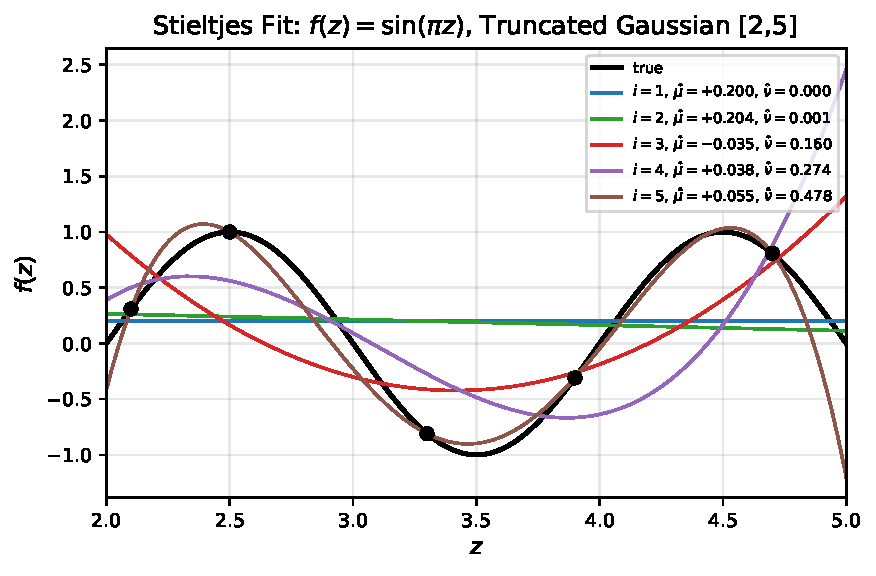
\includegraphics[width=\linewidth]{stieltjes_fit}
    \column{0.42\textwidth}
      \begin{block}{Setup}
        $f(z)=\sin(\pi z)$\\
        $z\sim\mathcal{N}(3,1)$ truncated to $[2,5]$\\
        True: $\mu\approx0.104$, $\nu\approx0.495$\\
        Samples: $\{2.1,2.5,3.3,3.9,4.7\}$
      \end{block}
      \begin{block}{Results by degree}
        \small
        \begin{tabular}{lrr}
          \toprule
          $i$ & $\hmu$ & $\hnu$\\
          \midrule
          1 & $+0.200$ & $-0.000$\\
          2 & $+0.204$ & $0.001$\\
          3 & $-0.036$ & $0.159$\\
          4 & $+0.037$ & $0.273$\\
          5 & $+0.055$ & $0.478$\\
          \bottomrule
        \end{tabular}
      \end{block}
      Higher degree captures more variance.
  \end{columns}
\end{frame}

\begin{frame}{Example 21.2 --- Hermite Chaos for Unknown Function}
  \begin{columns}[T]
    \column{0.52\textwidth}
      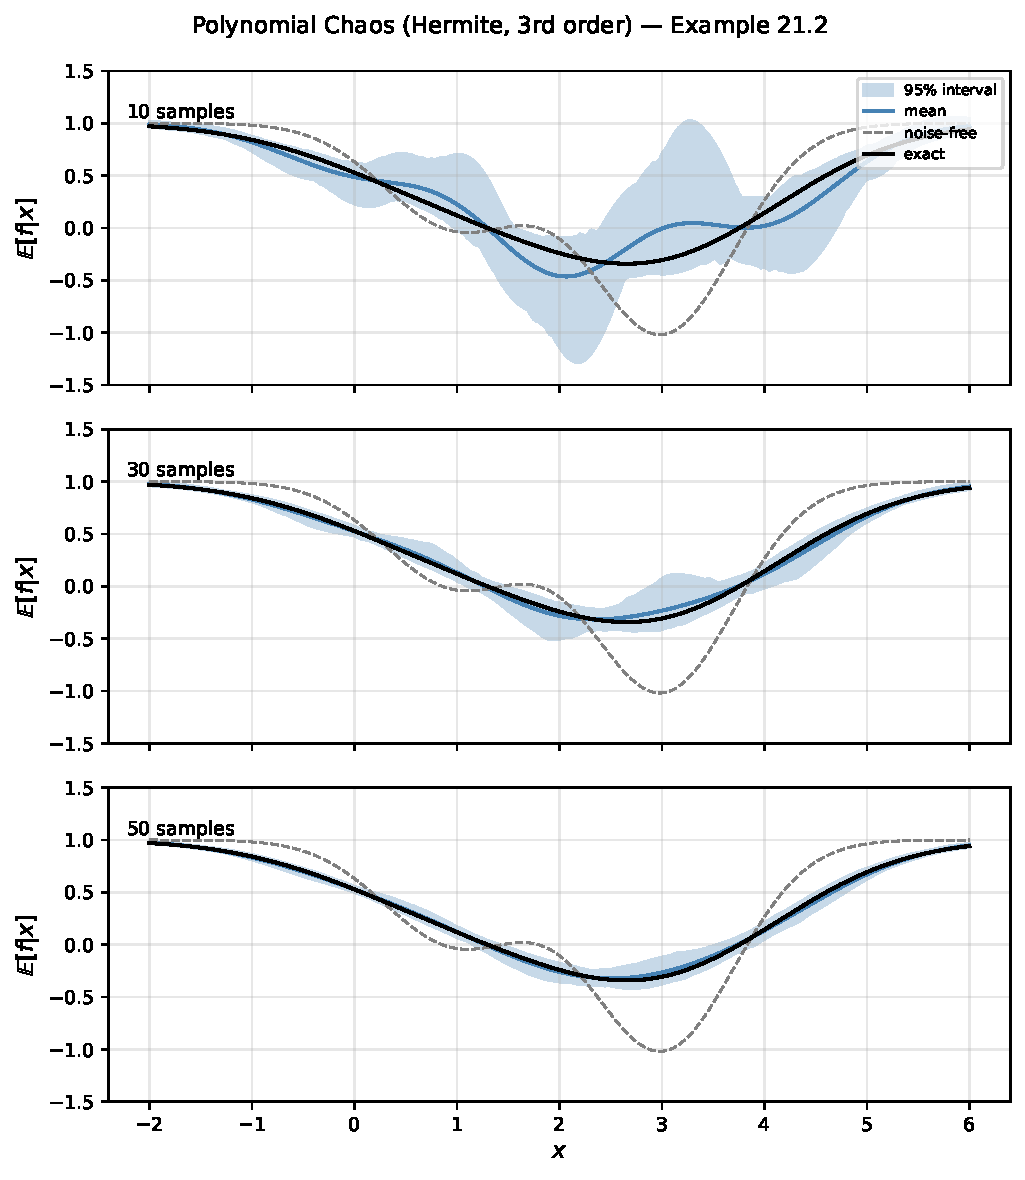
\includegraphics[width=\linewidth]{poly_chaos_hermite}
    \column{0.45\textwidth}
      \begin{block}{Setup}
        $f(x,z)=1-e^{-(x+z-1)^2}-2e^{-(x+z-3)^2}$\\
        $z\sim\mathcal{N}(0,1)$;
        3rd-order Hermite polynomials
      \end{block}
      \begin{block}{Observations}
        \begin{itemize}
          \item 10 samples: wide uncertainty
          \item 30 samples: mean starts tracking true
          \item 50 samples: good agreement with true expected value
        \end{itemize}
      \end{block}
      Blue band = 95\% bootstrap interval over repeated fits.
  \end{columns}
\end{frame}

\begin{frame}{21.3.3 Multivariate Polynomial Chaos}
  \begin{block}{Multivariate Basis via Product Construction (Eq.\ 21.39)}
    For $m$ random variables, multivariate basis functions are products
    of univariate bases:
    \[
      b_i(\bz) = \prod_{j=1}^{m} b_{a_j}(z_j)
    \]
    where $\mathbf{a}=[a_1,\ldots,a_m]$ is an \textbf{assignment vector}
    selecting the basis order for each dimension.
  \end{block}

  \begin{columns}[T]
    \column{0.48\textwidth}
      \begin{exampleblock}{Example 21.5 --- 3D basis}
        $b(\bz) = b_3(z_1)\,b_1(z_2)\,b_3(z_3)$\\
        assignment vector $\mathbf{a}=[3,1,3]$
      \end{exampleblock}
      The surrogate is still linear:
      $f(\bz)\approx\hf(\bz)=\sum_{i=1}^k\theta_i b_i(\bz)$
      and mean/variance formulas carry over.
    \column{0.48\textwidth}
      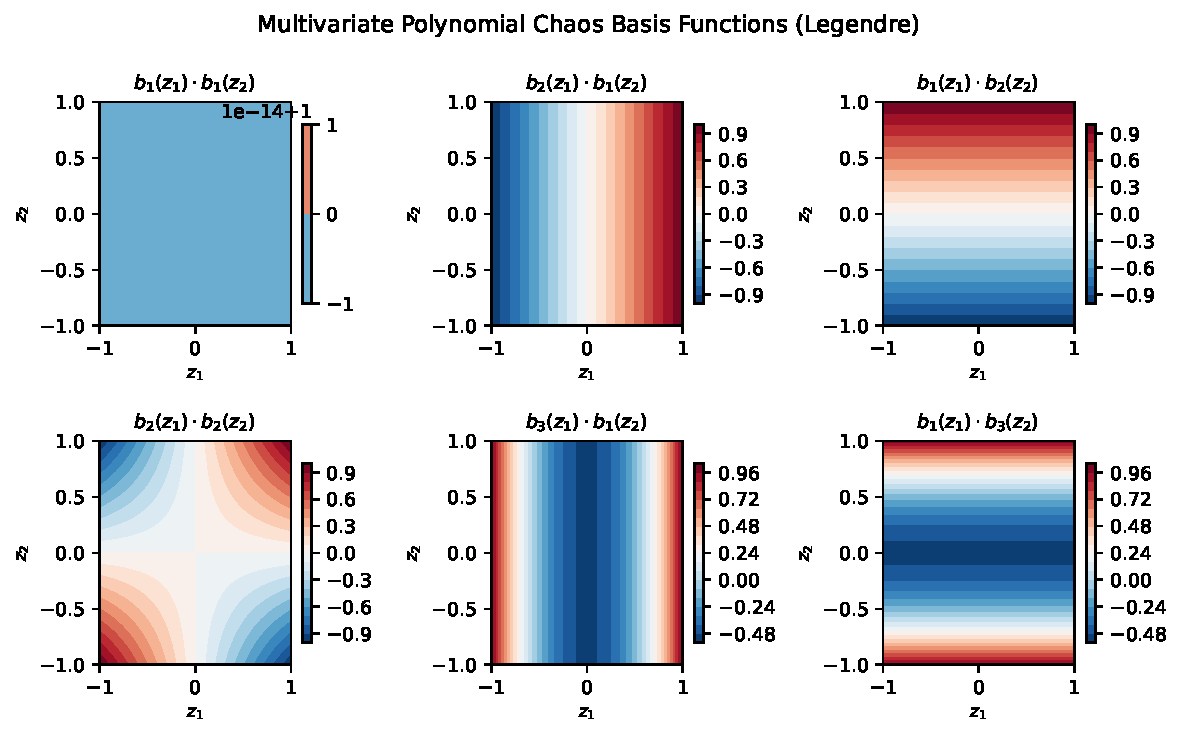
\includegraphics[width=\linewidth]{multivariate_basis}
      \begin{center}\small Legendre basis products for 2-D inputs\end{center}
  \end{columns}
\end{frame}

\begin{frame}[fragile]{Multivariate Polynomial Chaos in Python}
\begin{lstlisting}
import numpy as np
from itertools import product as iterproduct
from scipy.special import legendre as sp_legendre

def poly_chaos_bases_mv(bases_1d):
    """
    Build multivariate basis functions from 1-D bases.
    bases_1d : list of lists; bases_1d[j] = [b1_j, b2_j, ...] for variable j
    Returns  : list of callables, each mapping z (array) -> float
    """
    funcs = []
    for combo in iterproduct(*bases_1d):
        # combo = (b_{a_1}, b_{a_2}, ..., b_{a_m})
        def make_basis(c):
            return lambda z: np.prod([c[j](z[j]) for j in range(len(c))])
        funcs.append(make_basis(combo))
    return funcs

# Example: 2 variables, Legendre degree 0,1,2
bases_z1 = [sp_legendre(j) for j in range(3)]  # b1,b2,b3
bases_z2 = [sp_legendre(j) for j in range(3)]
mv_bases = poly_chaos_bases_mv([bases_z1, bases_z2])
print(f"Number of multivariate bases: {len(mv_bases)}")  # -> 9

# Evaluate at a point
z_test = np.array([0.5, -0.3])
vals = [b(z_test) for b in mv_bases]
print("Basis values:", np.round(vals, 4))
\end{lstlisting}
\end{frame}

% ============================================================
\section{21.4 Bayesian Monte Carlo}
% ============================================================

\begin{frame}{21.4 Bayesian Monte Carlo}
  \begin{columns}[T]
    \column{0.58\textwidth}
      \begin{block}{Idea}
        Use a \textbf{Gaussian process} (GP) --- a distribution over functions
        --- as a surrogate for $f$.
        Integrating over both the GP posterior and $p(\bz)$:
        \[
          \E_{\bz\sim p}[f] \approx
          \E_{\hf\sim p(\hf)}\!\left[\E_{\bz\sim p}[\hf]\right]
          = \int_{\mathcal{Z}} \hmu(\bz)\,p(\bz)\,d\bz
        \]
        where $\hmu(\bz)$ is the GP posterior mean (Eqs.\ 21.41--21.44).
      \end{block}
      \begin{block}{Variance of the estimate}
        \[
          \Var_{\bz\sim p}[f] \approx
          \int_{\mathcal{Z}}\!\int_{\mathcal{Z}}
          \mathrm{Cov}(\hf(\bz),\hf(\bz'))\,p(\bz)\,p(\bz')\,d\bz\,d\bz'
        \]
        where $\mathrm{Cov}(\hf(\bz),\hf(\bz')) = k(\bz,\bz') - k(\bz,Z)\mathbf{K}^{-1}k(Z,\bz')$
      \end{block}
    \column{0.38\textwidth}
      \begin{alertblock}{Also called}
        \textit{Bayes-Hermite Quadrature}
      \end{alertblock}
      \medskip
      \textbf{Advantages:}
      \begin{itemize}
        \item Encodes prior smoothness
        \item More efficient than MC for smooth $f$
        \item Analytic formulas when $\bz$ is Gaussian
      \end{itemize}
  \end{columns}
\end{frame}

\begin{frame}{Bayesian MC --- Gaussian Kernel, Gaussian Inputs}
  \begin{block}{Gaussian Kernel (Eq.\ 21.50)}
    \[
      k(\bz,\bz') = \exp\!\left(-\frac{1}{2}\sum_{i=1}^{n}
        \frac{(z_i-z'_i)^2}{w_i^2}\right), \quad
      \mathbf{W}=\mathrm{diag}[w_1^2,\ldots,w_n^2]
    \]
  \end{block}
  \begin{block}{Analytic Mean for $\bz\sim\mathcal{N}(\bmu_z,\bSigma_z)$ (Eq.\ 21.51)}
    \[
      \E_{\bz\sim p}[f] \approx \mathbf{q}^\top \mathbf{K}^{-1}\mathbf{y}
    \]
    \[
      q_i = \bigl|\mathbf{W}^{-1}\bSigma_z+\mathbf{I}\bigr|^{-1/2}
            \exp\!\left(-\tfrac{1}{2}(\bmu_z-\bz^{(i)})^\top
            (\bSigma_z+\mathbf{W})^{-1}(\bmu_z-\bz^{(i)})\right)
    \]
  \end{block}
  \begin{block}{Analytic Variance (Eq.\ 21.53)}
    \[
      \Var_{\bz\sim p}[f] \approx
      \bigl|2\mathbf{W}^{-1}\bSigma_z+\mathbf{I}\bigr|^{-1/2}
      - \mathbf{q}^\top\mathbf{K}^{-1}\mathbf{q}
    \]
  \end{block}
\end{frame}

\begin{frame}[fragile]{Bayesian Monte Carlo in Python --- Algorithm 21.5}
\begin{lstlisting}
import numpy as np

def gaussian_kernel(z1, z2, w):
    diff = np.asarray(z1) - np.asarray(z2)
    return np.exp(-0.5 * np.sum((diff / w)**2))

def build_K(Z, w):
    m = len(Z)
    return np.array([[gaussian_kernel(Z[i], Z[j], w)
                      for j in range(m)] for i in range(m)])

def bayesian_monte_carlo(Z, y, w, mu_z, Sigma_z):
    """
    Algorithm 21.5: Bayesian Monte Carlo with Gaussian kernel.
    Z      : (m, n) observed inputs
    y      : (m,)  observed function values
    w      : (n,)  kernel width parameters
    mu_z   : (n,)  Gaussian mean of uncertainty
    Sigma_z: (n,n) Gaussian covariance of uncertainty
    """
    W = np.diag(w**2)
    K = build_K(Z, w) + 1e-9 * np.eye(len(Z))
    invK = np.linalg.inv(K)
    # q vector
    SzpW_inv = np.linalg.inv(Sigma_z + W)
    det_fac = np.linalg.det(np.linalg.inv(W) @ Sigma_z + np.eye(len(w)))
    q = np.array([np.exp(-0.5*(mu_z-z)@SzpW_inv@(mu_z-z)) for z in Z])
    q *= det_fac**(-0.5)
    mu_est = q @ invK @ y
    nu_est = (np.linalg.det(2*np.linalg.inv(W)@Sigma_z + np.eye(len(w)))**(-0.5)
              - q @ invK @ q)
    return mu_est, nu_est
\end{lstlisting}
\end{frame}

\begin{frame}{Example 21.6 --- Bayesian MC vs Sample Mean}
  \begin{columns}[T]
    \column{0.55\textwidth}
      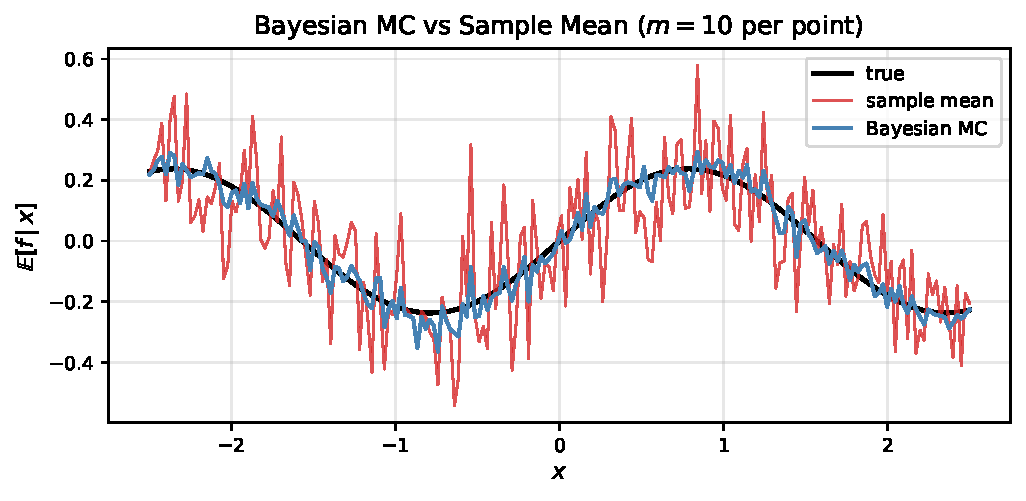
\includegraphics[width=\linewidth]{bayesian_mc}
    \column{0.42\textwidth}
      \begin{block}{Setup}
        $f(x,z)=\sin(x+z_1)\cos(x+z_2)$\\
        $z_1\sim\mathcal{N}(0,1)$, $z_2\sim\mathcal{N}(0,0.5)$\\
        $\bmu_z=[0,0]$, $\bSigma_z=\mathrm{diag}[1,0.5]$\\
        Kernel weights $\mathbf{w}=[1,1]$\\
        $m=10$ samples per $x$
      \end{block}
      \begin{block}{Key Result (at $x=0$)}
        $\mathbf{K}$ matrix computed from 5 samples\\
        $\mathbf{q}=[0.577,0.450,0.450,0.417,0.417]$\\
        $\E[f]=0.0$, $\Var[f]=0.327$
      \end{block}
      Bayesian MC is \textbf{much smoother} than raw sample mean.
  \end{columns}
\end{frame}

% ============================================================
\section{Method Comparison}
% ============================================================

\begin{frame}{Method Comparison}
  \begin{center}
    
\includegraphics[width=0.85\linewidth]{method_comparison}
  \end{center}
  \vspace{-0.5em}
  \begin{center}\small Mean estimates for $f(x,z)=\sin(x+z_1)\cos(x+z_2)$\end{center}
\end{frame}

\begin{frame}{Methods at a Glance}
  \small
  \begin{center}
  \begin{tabular}{p{2.5cm}p{3.5cm}p{3.5cm}p{2.5cm}}
    \toprule
    \textbf{Method} & \textbf{Assumptions} & \textbf{Pros} & \textbf{Cons}\\
    \midrule
    Monte Carlo & None & Simple; black-box & Slow convergence $\mathcal{O}(m^{-1/2})$\\[4pt]
    Taylor Approx. & $f$ smooth, small $\nu_i$ & Analytic; no samples & Needs derivatives; poor for nonlinear $f$\\[4pt]
    Polynomial Chaos & $f$ approx.\ polynomial & Efficient once bases fixed; analytic $\hmu,\hnu$ & Exponential growth in variables\\[4pt]
    Bayesian MC & $f$ smooth; GP prior & Very efficient; encodes prior & GP fitting overhead\\
    \bottomrule
  \end{tabular}
  \end{center}
\end{frame}

% ============================================================
\section{21.5 Summary \& Exercises}
% ============================================================

\begin{frame}{21.5 Summary}
  \begin{itemize}
    \setlength{\itemsep}{0.5em}
    \item The \textbf{expected value} and \textbf{variance} of the objective
          function are useful when optimizing under uncertainty; computing them
          reliably can be challenging.

    \item \textbf{Monte Carlo integration} is the simplest approach:
          estimate moments by averaging function evaluations over random samples.
          Convergence rate is $\mathcal{O}(m^{-1/2})$.

    \item The \textbf{Taylor approximation} uses partial derivatives to
          analytically approximate the mean and variance; first- and second-order
          versions are available.

    \item \textbf{Polynomial chaos} fits an orthogonal polynomial surrogate
          to observed data; the mean equals the first coefficient $\theta_1$
          and the variance follows from the squared higher-order coefficients.

    \item \textbf{Bayesian Monte Carlo} uses Gaussian processes as surrogates;
          analytic formulas for Gaussian kernels and Gaussian inputs make it
          especially powerful.

    \item For \textbf{multivariate} inputs, polynomial chaos uses a product
          construction; the number of basis functions grows exponentially
          in the number of variables.
  \end{itemize}
\end{frame}

\begin{frame}{21.6 Exercises --- Overview}
  \begin{block}{Exercise 21.1}
    $z\sim\mathcal{N}(0,1)$.
    Show: $P(|z|\le 1)\approx 68.3\%$;\;
    $P(z\le 1)\approx 84.1\%$.
    \textit{Hint: use the CDF of the standard normal.}
  \end{block}

  \begin{block}{Exercise 21.2}
    Let $x^{(1)},\ldots,x^{(m)}$ be i.i.d.\ with mean $\mu$, variance $\nu$.
    Show $\Var(\hmu)=\nu/m$.
    \textit{Key: $\Var(\sum a_i X_i) = \sum a_i^2 \Var(X_i)$ for independent $X_i$.}
  \end{block}

  \begin{block}{Exercise 21.3}
    Derive the three-term recurrence relation (Eq.\ 21.29) from first principles.
    \textit{Key: use the shift property $\int(z b_i)b_j\,p\,dz = \int b_i(z b_j)\,p\,dz$.}
  \end{block}

  \begin{block}{Exercise 21.4}
    Derive an expression for $\partial\theta_j/\partial x_i$ using pseudo-inverse.
    Approximate: $[\partial\bm{\theta}/\partial x_i]
    \approx \mathbf{B}^{+}[\partial f/\partial x_i]_{\text{at samples}}$.
  \end{block}
\end{frame}

\begin{frame}{Exercise 21.5 --- Gradient of $f_{\text{mod}}$ via Polynomial Chaos}
  \begin{block}{Problem}
    The modified objective under uncertainty (Ch.~20):
    $f_{\text{mod}}(\bx,\bz) = \alpha\hmu(\bx) + (1-\alpha)\hnu(\bx)$

    Derive $\partial f_{\text{mod}}/\partial x_i$ using polynomial chaos.
  \end{block}

  \begin{block}{Solution}
    The chaos estimates satisfy:
    \[
      \hmu(\bx) = \theta_1(\bx),\qquad
      \hnu(\bx) = \sum_{i=2}^{k}\theta_i^2(\bx)\int_{\mathcal{Z}} b_i(z)^2 p(z)\,dz
    \]
    Therefore:
    \[
      \frac{\partial f_{\text{mod}}}{\partial x_i}
      = \alpha\frac{\partial\theta_1}{\partial x_i}
        + 2(1-\alpha)\sum_{j=2}^{k}\theta_j(\bx)
          \frac{\partial\theta_j}{\partial x_i}
          \int_{\mathcal{Z}} b_j(z)^2 p(z)\,dz
    \]
    Coefficient gradients $\partial\theta_j/\partial x_i$ are estimated
    from Exercise 21.4 using the pseudo-inverse.
  \end{block}
\end{frame}

% ============================================================
\section*{Appendix: Python Reference}
% ============================================================

\begin{frame}[fragile,allowframebreaks]{Full Python Example: All Methods Compared}
\begin{lstlisting}
import numpy as np
from scipy.special import legendre as sp_legendre

# -- Setup --------------------------------------------------
np.random.seed(42)
# f(x=0, z) = sin(z1)*cos(z2), z1~N(0,0.1), z2~N(0,0.2)
x = 0.0
def f(z): return np.sin(x + z[0]) * np.cos(x + z[1])
mu_z = np.array([0.0, 0.0])
nu_z = np.array([0.1, 0.2])

# -- Monte Carlo --------------------------------------------
m = 2000
Z = np.column_stack([np.random.randn(m)*np.sqrt(0.1),
                     np.random.randn(m)*np.sqrt(0.2)])
fz = np.array([f(Z[i]) for i in range(m)])
mu_mc = np.mean(fz)
nu_mc = np.mean(fz**2) - mu_mc**2
print(f"Monte Carlo (m={m}): mu={mu_mc:.4f}, nu={nu_mc:.4f}")

# -- Taylor Approximation (1st order) ----------------------
# df/dz1|z=0 = cos(x)^2, df/dz2|z=0 = -sin(x)^2
eps = 1e-5
e1 = np.array([eps, 0.0]); e2 = np.array([0.0, eps])
g1 = (f(mu_z+e1) - f(mu_z-e1)) / (2*eps)
g2 = (f(mu_z+e2) - f(mu_z-e2)) / (2*eps)
mu_ta = f(mu_z)
nu_ta = g1**2 * nu_z[0] + g2**2 * nu_z[1]
print(f"Taylor 1st order:     mu={mu_ta:.4f}, nu={nu_ta:.4f}")

# -- Polynomial Chaos (Legendre, univariate on z1 only) ----
# Marginalize: ignore z2 for illustration
z_s = np.linspace(-1, 1, 20)
y_s = np.array([f([z, 0.0]) for z in z_s])
k = 4
B = np.column_stack([sp_legendre(j)(z_s) for j in range(k)])
theta, _, _, _ = np.linalg.lstsq(B, y_s, rcond=None)
mu_pc = theta[0]
nu_pc = sum(theta[j]**2 / (2*j+1) for j in range(1, k))
print(f"Polynomial Chaos (k={k}): mu={mu_pc:.4f}, nu={nu_pc:.4f}")
\end{lstlisting}
\end{frame}

\begin{frame}{Key Formulas at a Glance}
  \begin{columns}[T]
    \column{0.48\textwidth}
      \begin{block}{Monte Carlo}
        $\hmu = \tfrac{1}{m}\sum f(\bz^{(i)})$\\
        $\hnu = \tfrac{1}{m}\sum f(\bz^{(i)})^2 - \hmu^2$\\
        $\Var[\hmu] = \nu/m$
      \end{block}
      \medskip
      \begin{block}{Taylor (1st order)}
        $\hmu = f(\bmu_z)$\\
        $\hnu = \sum_i (\partial f/\partial z_i)^2 \nu_i$
      \end{block}
    \column{0.48\textwidth}
      \begin{block}{Polynomial Chaos (orthogonal)}
        $f(z)\approx\sum_i\theta_i b_i(z)$\\
        $\hmu = \theta_1$\\
        $\hnu = \sum_{i=2}^k\theta_i^2\int b_i^2 p\,dz$
      \end{block}
      \medskip
      \begin{block}{Bayesian MC (Gaussian)}
        $\E[f]\approx\mathbf{q}^\top\mathbf{K}^{-1}\mathbf{y}$\\
        $\Var[f]\approx|2\mathbf{W}^{-1}\bSigma_z{+}\mathbf{I}|^{-1/2}
         -\mathbf{q}^\top\mathbf{K}^{-1}\mathbf{q}$
      \end{block}
  \end{columns}
\end{frame}

\end{document}
